\begin{landscape}
\chapter{Knowledge Flows}
\label{chap:knowledgeflows}

\begin{figure}[H]
\centering
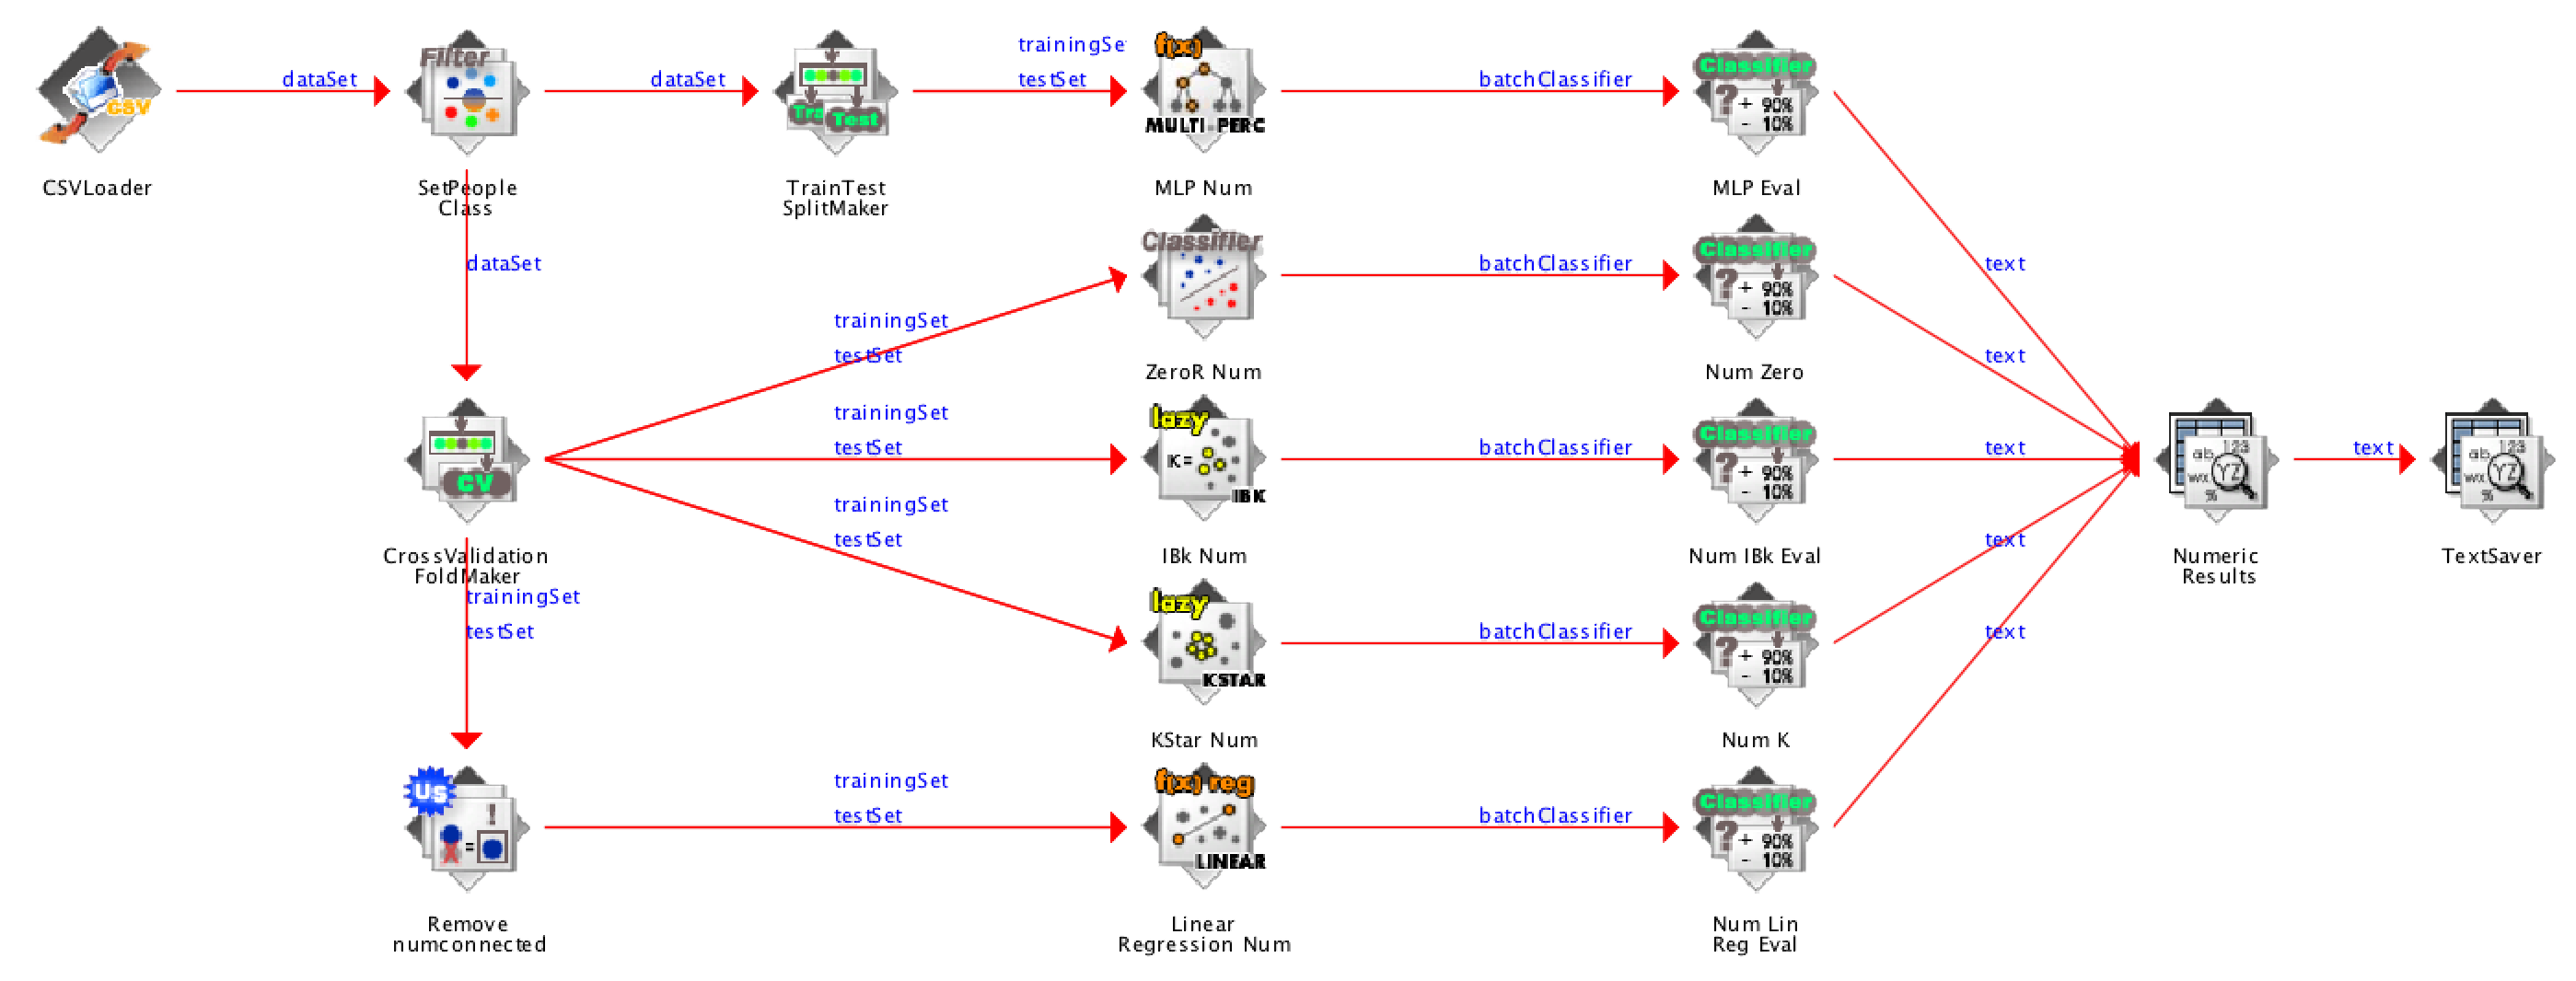
\includegraphics[width=\linewidth]{../diagrams/knowledgeflow-numeric.png}
\caption{Numeric knowledge flow}
\end{figure}
\end{landscape}

\begin{landscape}
\begin{figure}[H]
\centering
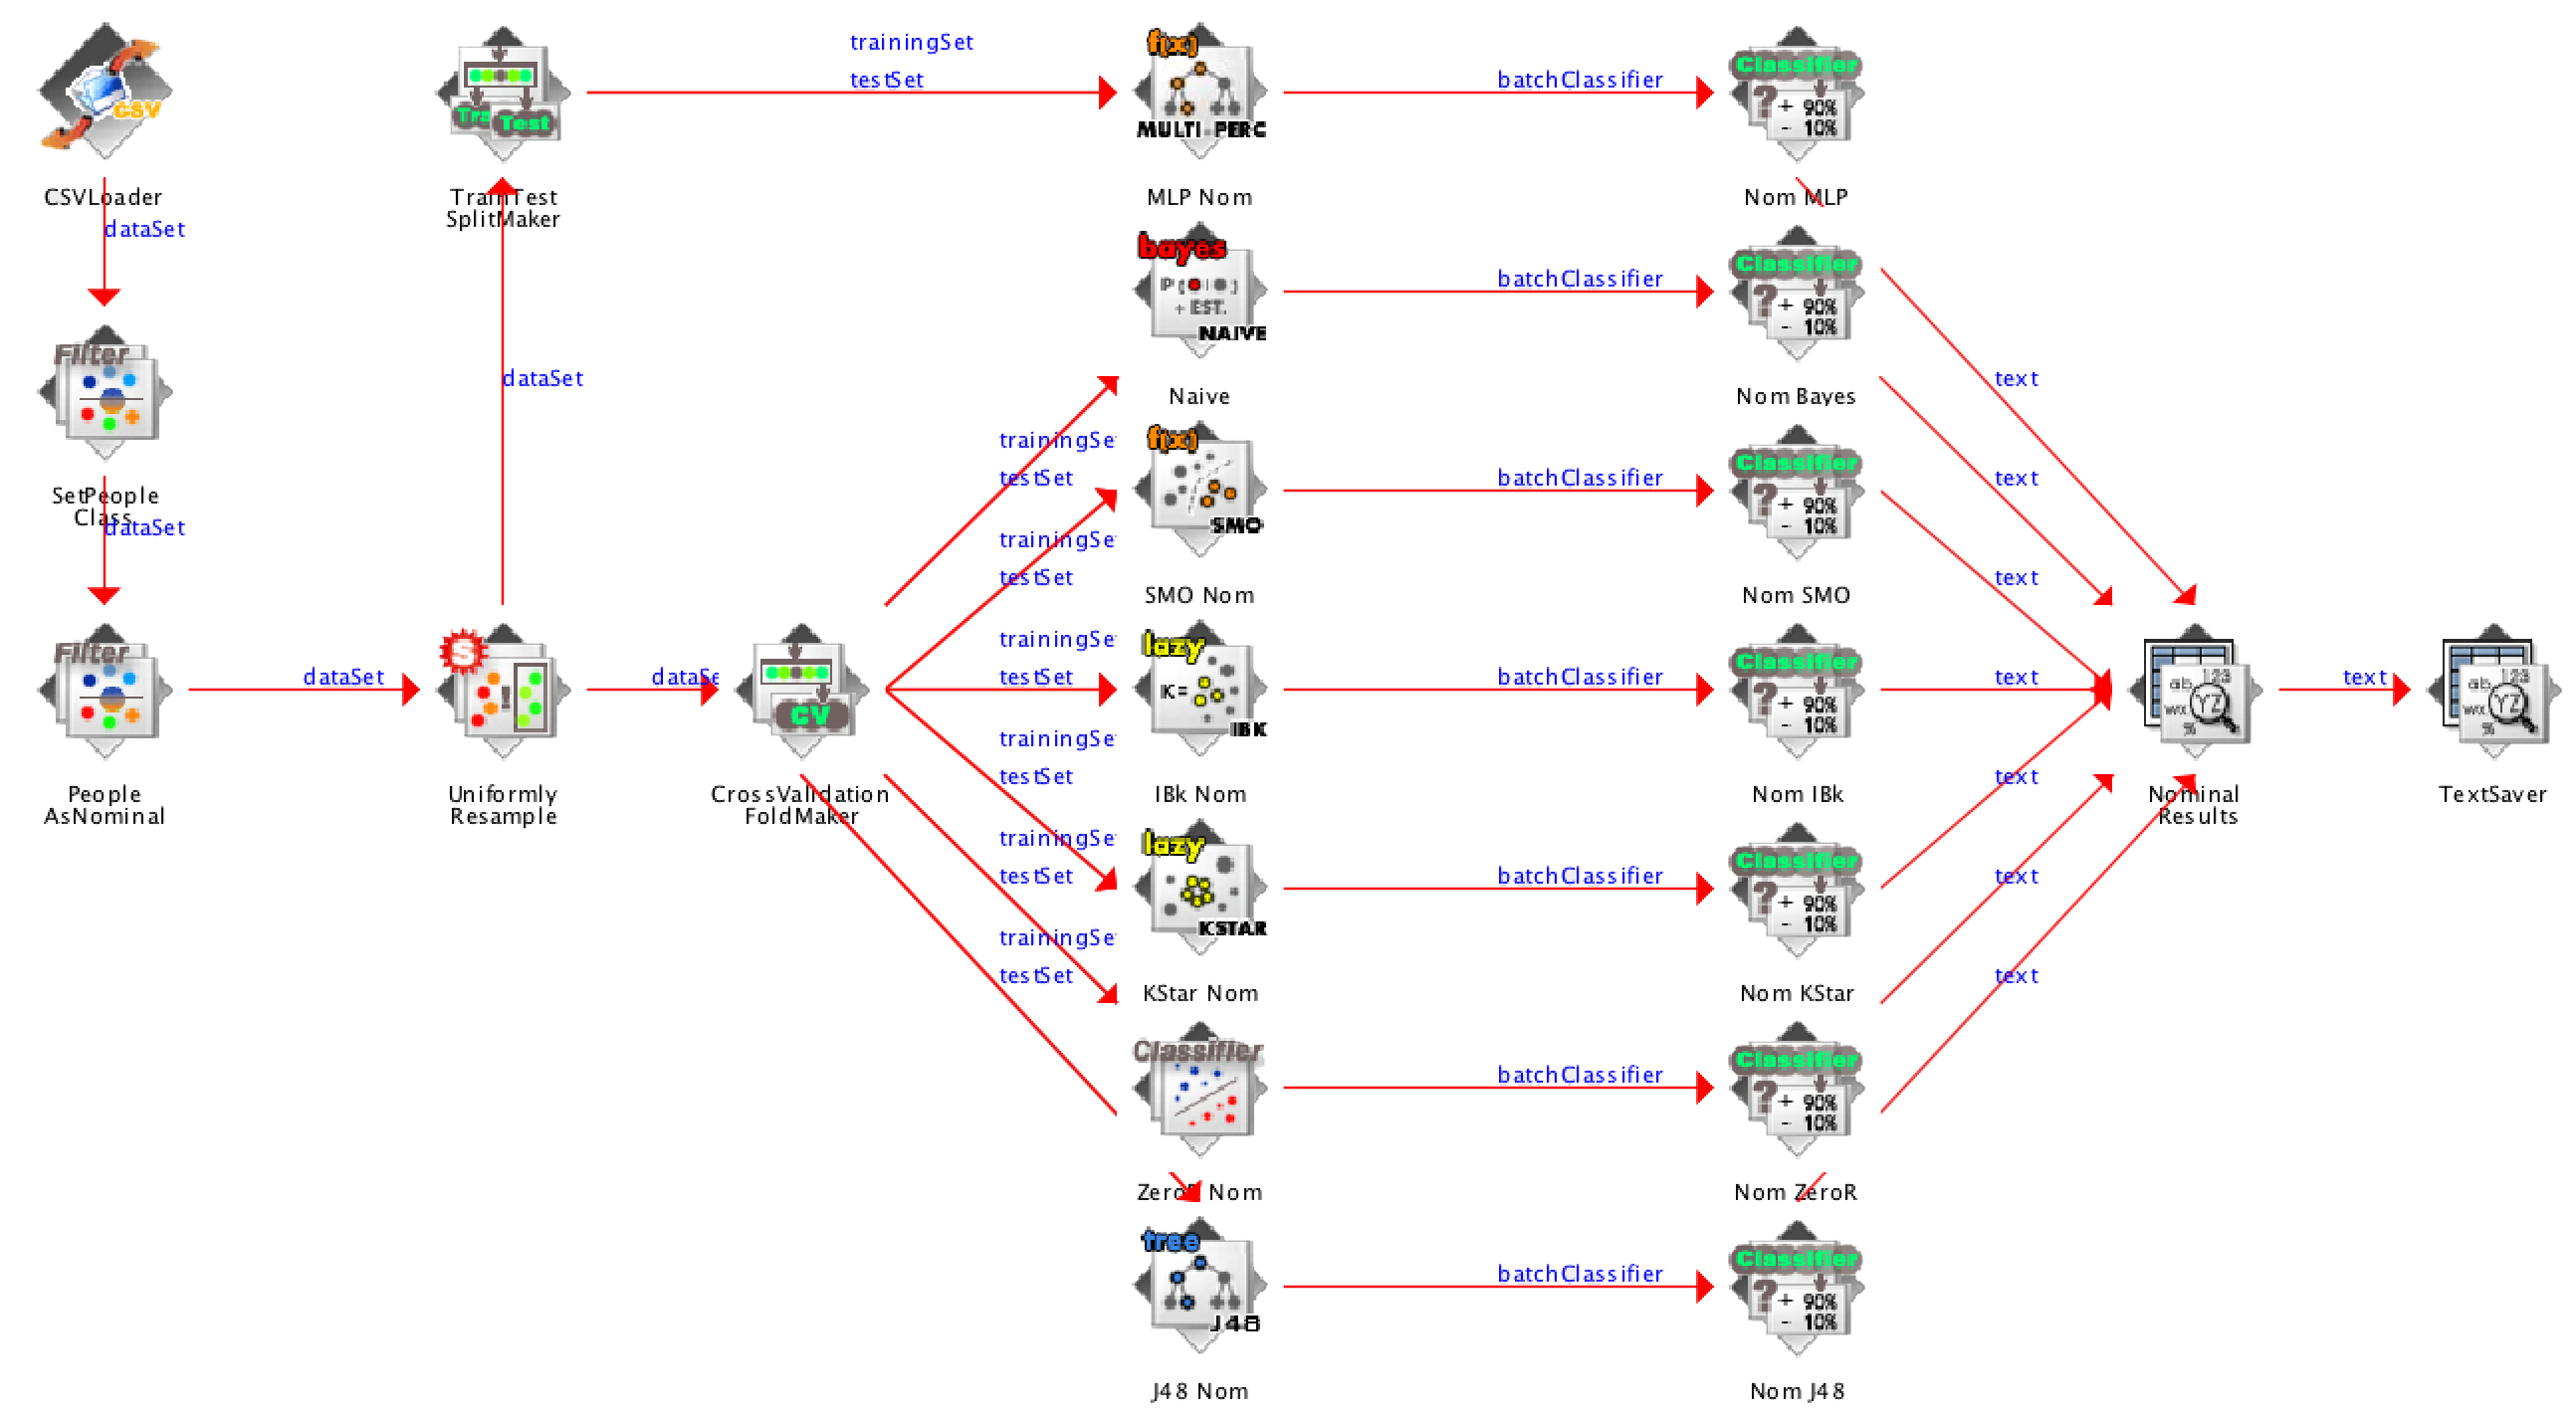
\includegraphics[width=\linewidth]{../diagrams/knowledgeflow-nominal.png}
\caption{Nominal knowledge flow}
\end{figure}

In Weka, Knowledge Flows can be defined, which provide an easy way to replicate a series of Weka functions. We provide a unified knowledge flow at the \texttt{run\_flow.py} script to execute it on a given data set. However, we also replicate the numeric and nominal flows here (separated due to size) for those interested.
\end{landscape}

\chapter{Original Honours Proposal}
\subfile{../proposal/proposal}